We will discuss two kinds of algebro-geometric objects that have Berkovich spaces associated to them. 
The first one is the analytification of a variety over $K$, analogous to analytification of complex varieties like we discussed at the start of this chapter. 
The second is that there is a natural interpretation of the formal fiber of a formal scheme over $R = \mathcal{O}_K = \{a \in K \st |a| \le 1\} $ as a Berkovich space. 


\subsection{Analytification of Varieties} \label{sec:analytfication_of_varieties}


Suppose $X$ be a scheme, locally of finite type over $K$.  We want define an analytification functor that takes such schemes to $K$-analytic spaces.  
\begin{definition}
	Let  $X$ be a locally finite $K$-scheme. 
	The \emph{analytification of $X$} is the pair $(X\an, i: X\an \to X)$ a $K$-analytic space $X\an$ together with a morphism of ringed spaces $i: X\an \to X$, satisfying the following universal property:
	For any good $K$-analytic space $Y$ and morphism of locally ringed spaces $f: Y \to X$, the map $f$ factors uniquely through $i: X\an \to X$. 
	\[
	\begin{tikzcd}
		 & X\an \dar{i} \\
		Y \rar{f} \ar[dashed]{ur}{\exists !} & X
	\end{tikzcd}
	.\] 
\end{definition}
So $X\an$ represents the functor from $K$-analytic spaces $Y \mapsto \hom(Y, X)$ where the hom-set is in the category of locally ringed spaces. 
\nomenclature[an]{$X\an$}{The Berkovich analytification of $X$}

This universal property is good for theoretical purposes, but in practice it is nice to have an more concrete understanding of the analytification of a $K$-variety. 
\begin{definition}\label{def:berkovich_analytification_explicit}
	The \emph{Berkovich analitification} of a locally finite type scheme $X$ over  $K$, as a set is \[
		X\an = \{(x, |\cdot |)  \mid x\in X, |\cdot | \text{ a norm on } \kappa(x) \text{ extending the norm on }K \} 
	.\] 

	This comes equipped with a canonical projection map $i: X\an \to X, (x, |\cdot |) \mapsto  x$.
	
	$X\an $ comes with a topology which we define to be the coarsest topology such that 
	\begin{itemize}
		\item $i: X\an \to X$ is continuous, i.e. $X\an$ is a finer space than  $X$. 
		\item For every open $U \subset X$ and $f \in \mathcal{O}_X(U)$ the map  \[
				|f|: i^{-1}(U) \to \R^{+}: (x, |\cdot |) \mapsto  |f(x)|
		\] 
		is continuous.
	\end{itemize}

\end{definition}

\begin{remark}
	If $X$ is an affine scheme $X = \spec A$ over $K$, then this construction agrees with our adhoc definition from \cref{sec:berkovich_spaces}
	by mapping a norm $x \in \mathcal{M} (A)$ onto $(\ker x, x')$ where $x'$ is the norm on $\kappa(\ker x)$ induced by $x$. 
	\[
		X^{\an} = \mathcal{M} (A)
	\] 

	We will continue to write $\mathcal{M} (A)$ for the Berkovich analytification of $\spec A$, only this time it includes the structure sheaf. 
\end{remark}



\begin{example}[The Berkovich affine line $\aff^{1, \text{an}}_K$]\label{ex:affine_line_union_disks}
	We already discussed the topology of $\aff^{1, \text{an}}_K$ in \cref{sec:the_berkovich_spectrum_of_z}. 
	But we can now discuss how $\aff^{1, \text{an}}$ behaves as a $K$-analytic space as well. 

	For any $r$ there is a natural inclusion $K[T] \into K\left<r^{-1} T \right>$ and this inclusion is dense. 
	Hence any (semi)norm on $K\left<r^{-1}T \right>$ is uniquely determined by its restriction to $K[T]$.
	Conversely any (semi)norm $|\cdot |_x$ on  $K[T]$ extends to a bounded (semi)norm $K\left<r^{-1}T \right>$ if and only if $r^{-1}|T|_x < 1$, i.e. $|T|_x \le r$. 

	This shows (that as sets at least)
	\[
		\aff^{1, \text{an}}_K = \bigcup_{r = 1} ^{\infty} \mathcal{M} (K\left<r^{-1} T \right>)
	.\] 

\begin{figure}[ht]
    \centering
    \incfig{affine-line-as-union-of-disks}
    \caption{Affine line as union of disks}
    \label{fig:affine-line-as-union-of-disks}
\end{figure}
\end{example}

\begin{example}
	\Cref{ex:affine_line_union_disks} can actually be extended to see how any variety might be analytified. 
	Lets start with affine varieties. 
	First note that for higher dimensional ($\dim X = d$) affine space $\aff_K^{d}$ can be analytified by an increasing union of disks \[
		\aff_K^{d, \text{an}} = \bigcup_{r = 1} ^{\infty} \mathcal{M} \left(K \left<r^{-1} T_1, \ldots, r^{-1} T_d \right>\right)
	.\] 
	Let $A = K[T_1,\ldots, T_n] / (f_1, \ldots, f_m)$ be any finite type scheme, and consider the closed immersion $f: \spec A \to \aff_K^{n} = \spec (K[T_1, \ldots, T_n]) $. 
	Then for any affinoid algebra $A_V$ and morphism $\mathcal{M} (A_V) \to \spec A$ gives a morphism to $\aff_K^{n, \text{an}}$ lying in the zero set cut out by $f_1, \ldots, f_n$. Hence they factor uniquely over algebras of the type $K \left<r^{-1} T_1, \ldots, r^{-1} T_n \right>/ (f_1, \ldots, f_n)$. 
	So \[
		\spec A \an = \bigcup_{r= 1} ^{\infty} \mathcal{M} \left(\frac{K \left<r^{-1} T_1, \ldots, r^{-1} T_n \right>}{(f_1, \ldots, f_n)}\right)
	.\] 
	For general varieties one can consider an affine cover by finite type algebras and glue their analytification. 
	For a more detailed exposition of this construction see \cite[sec.\ 3.4]{berkovichSpectralTheoryAnalytic2012}. 
\end{example}

\begin{example}
	[Berkovich Projective line]
	We can construct the analytification of $\pro^{1}_K$ in the same way as one might construct the scheme $\pro^{1}_K$ by gluing together two copies of the affine line. 
	So we first find analytification on an affine cover $K[T], K[T^{-1}]$ and glue the spaces $\mathcal{M} (K[T]), \mathcal{M} (K[T^{-1})$ along $\mathcal{M} (K[T, T^{-1}])$. 
Using the description in \cref{def:berkovich_analytification_explicit} we see that $\mathcal{M} (K[T, T^{-1}]) = \aff^{1, \text{an}}_K \setminus \{0\} $.
See \cref{fig:berk_projective_line}. 
\end{example}

\begin{figure}[h]
	\centering
	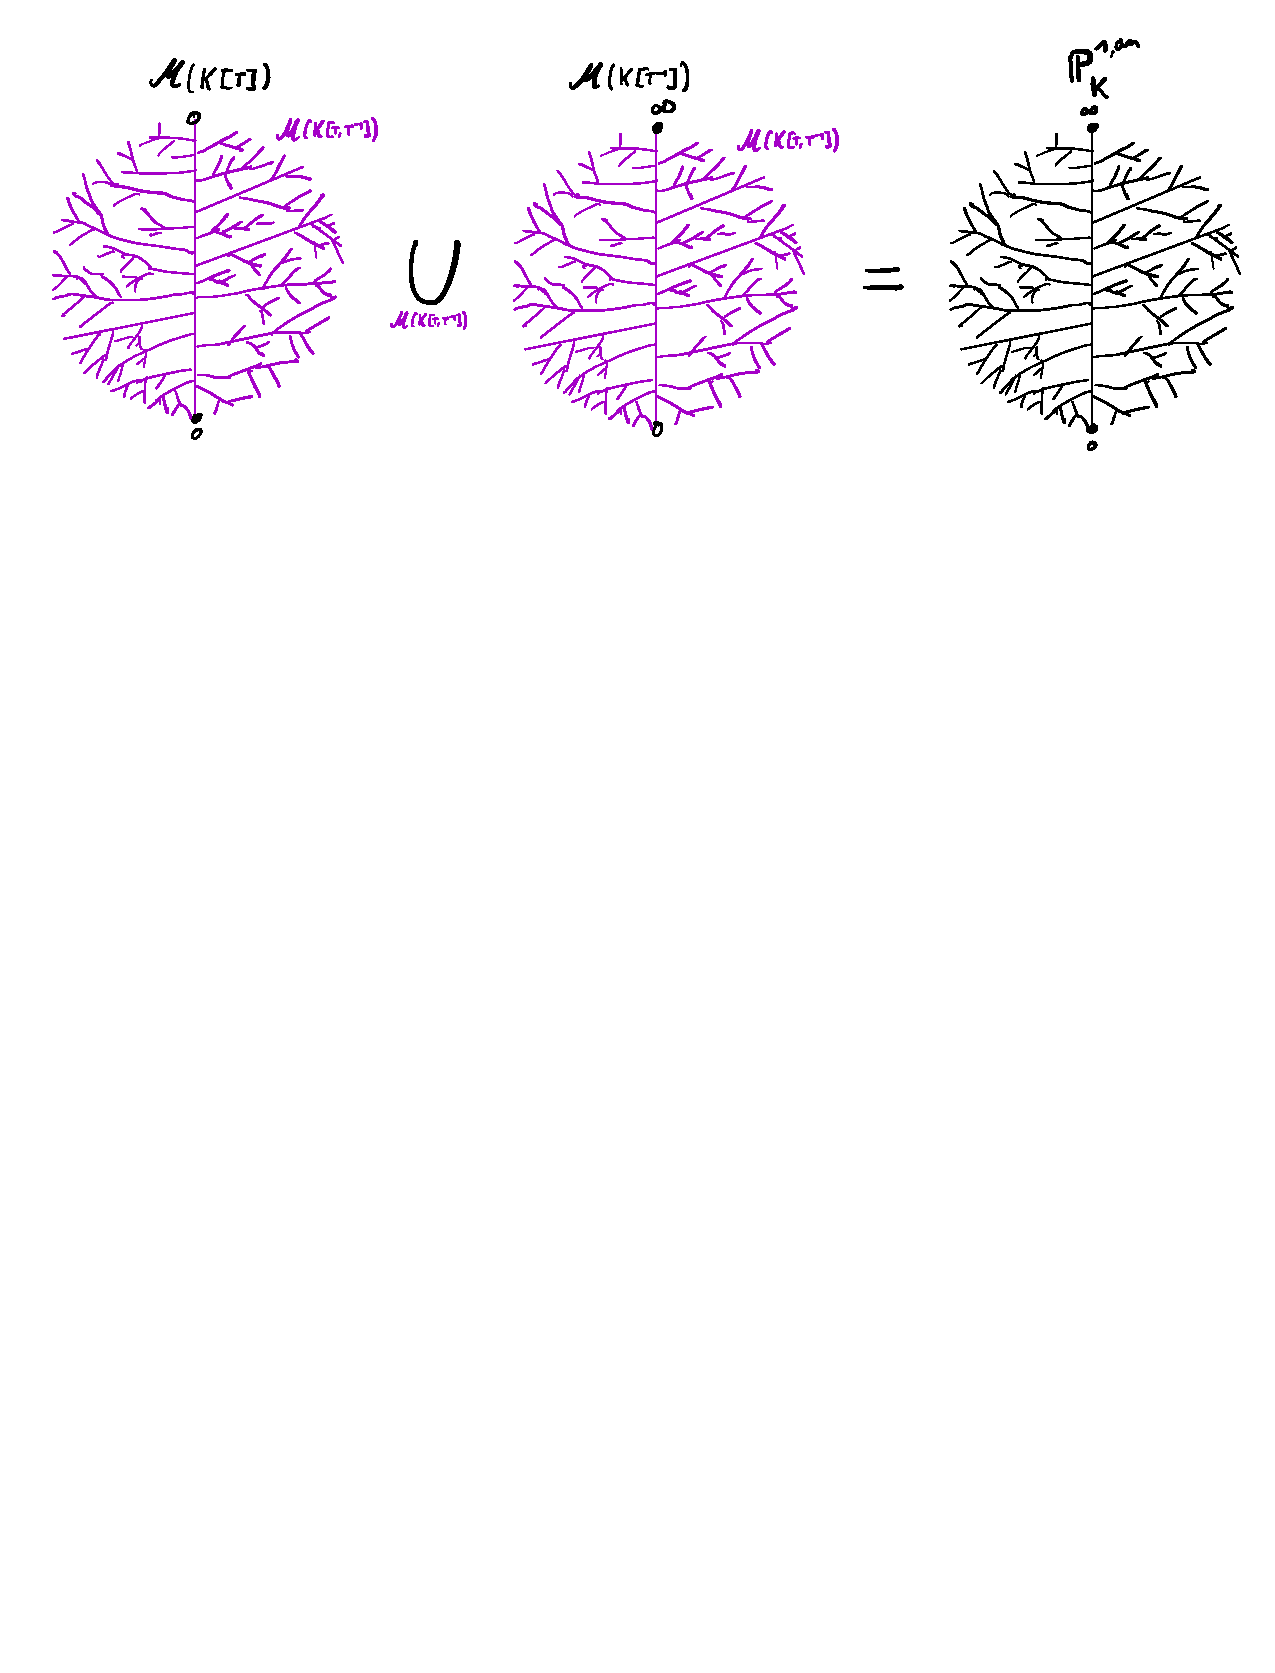
\includegraphics[width=\textwidth]{figures/projective_line}
	\caption{The Berkovich projective line constructed by gluing two copies of $\aff^{1, \text{an}}_K$}
	\label{fig:berk_projective_line}
\end{figure}


Like the analytification of complex varieties there are certain GAGA results, which show that under specific conditions all information is preserved by passing to the Berkovich analytification. 
Once one has setup the right definitions of smooth, flat, unramified, étale and open immersion for $K$-analytic spaces (see \cite[][sec. 3.1]{berkovichSpectralTheoryAnalytic2012} for definitions) one can show the following:
\begin{theorem}
	Let $f: Y \to X$  be a morphism of $K$-varieties. Then $f\an: Y \an \to X\an$ has any of the following properties if and only $\phi$ has: flat, unramified, étale, smooth, separated, injective, surjective, open immersion, isomorphism and monomorphism. 

	If moreover $f$ is a morphism of finite type then the following may be added to the list: dominant, closed immersion, proper and finite. 
\end{theorem}
\begin{proof}
	See \cite[][prop.\ 3.4.6 and prop.\ 3.4.7]{berkovichSpectralTheoryAnalytic2012}
\end{proof}

\begin{theorem}
	The topology of $X\an$ reveals a lot of the ``topological'' properties of the scheme $X$. 
	\begin{itemize}
		\item $X$ is separated if and only if $X\an$ is Hausdorff. 
		\item $X$ is proper if and only if $X\an$ is Hausdorff and compact. 
		\item  $X$ is connected if and only if $X\an$ is path-connected. 
		\item The Krull dimension of  $X$ is equal to the topological dimension of $X\an$. 
	\end{itemize}
\end{theorem}
\begin{proof}
	See \cite[][thm.\ 3.4.8]{berkovichSpectralTheoryAnalytic2012}
\end{proof}

For more on the GAGA results see \cite[][sec.\ 3.4]{berkovichSpectralTheoryAnalytic2012}.

\subsection{Generic fiber of a formal scheme} \label{sec:generic_fiber_of_a_formal_scheme}

Recall that $R = \mathcal{O}_K = \{a \in K \mid |a| \le 1\} $, which is a topological ring with the metric induced by the norm. 
Let $\pi$ be a pseudo-uniformiser for $R$ and $I = (\pi)$. 
Then $\{I^{n}\}_n$ gives a system of neighborhoods around zero, and $R$ is complete with respect to this topology. 
This means that $R$ is an adic ring, which is useful if we want to use the language of formal schemes. 

We first need to restrict the class of rings and formal schemes we consider. 
\begin{definition}\label{def:topologically_finite_presentation_algebra}
	\begin{itemize}
		\item 
	A \emph{topologically finitely presented} $R$-algebra is a quotient \[
		R\left<x_1, \ldots, x_n \right> / \mathfrak{a} 
	,\] where $\mathfrak{a}  = (f_1, \ldots, f_m)$ is a finitely generated ideal. 
\item A formal scheme that is locally isomorphic to $\spf A$ for some topologically finite presented $R$-algebra is called a \emph{locally finite type} $R$ formal scheme. 
	\end{itemize}

\end{definition}

Given such a topologically finitely presented ring $A = \frac{R \left<x_1, \ldots, x_n \right>}{(f_1, \ldots, f_m)}$ we can tensor it with $K$ to get its ``generic fiber'' which is an affinoid algebra \[
A \otimes _R K = \frac{K \left<x_1, \ldots, x_n \right>}{(f_1, \ldots, f_m)}
.\]  
This suggest the following functor $\spf A \mapsto \mathcal{M} (A \otimes_R K)$. 
Indeed this functor glues to give a functor from the topologically finitely presented $R$ formal schemes to the category of $K$-analytic spaces. 

\begin{definition}\label{def:generic_fibre_of_formal_scheme}
Given a topologically finitely presented formal schemes $\mathfrak{X} $ we call the resulting $K$-analytic space the \emph{generic fibre of  $\mathfrak{X} $} and denote it by $\mathfrak{X} _\eta$. 
\end{definition}

\begin{definition}
	Let $X$ be a $K$-variety. 
	\begin{itemize}
		\item A formal model of $X$ is a locally finite type formal $R$-scheme together with an isomorphism $X\an \cong \mathfrak{X}_{\eta}$.
		\item A formal model $\mathfrak{X}  $ of $X$ is \emph{semistable} if its special fiber $\mathfrak{X} _s = \mathfrak{X} \times_R \spec k$ is a connected reduced curve whose singularities are ordinary double points. 
	\end{itemize}
\end{definition}

\begin{comment}
Later we will extend the construction of the generic fiber to the larger class of \emph{special formal schemes}.
These will be really useful for understanding the relation between formal models of curves and their Berkovich space. 
\begin{definition}\label{def:special_r_algebra}
	A \emph{special} $R$-algebra is a $R$-algebra of the form \[
		\frac{A\left<x_1, \ldots, x_n \right>[[y_1, \ldots, y_m]]}{(f_1, \ldots, f_\ell)}
	.\] 
\end{definition}
\end{comment}





